\begin{frame}[fragile]
\frametitle{Ancient Mathematics}
\begin{itemize}[label=\textbullet,noitemsep,nolistsep]
\item \textbf{Number Systems}:
	\begin{itemize}[label=\textbullet, noitemsep,nolistsep]
	\item Base 5 (Quinary): Easy to use with just one hand
	\item Base 60 (Sexagesimal): Sumerian/Babylonian
	\end{itemize}
\item \textbf{Egyptians}: Trigonometry, Ratios, $\pi$ (Pyramid)
\item \textbf{Arabic}: Al-gebra (without negatives), Astronomy (planet positions to find {\it namaaz} times)
\item \textbf{Omar Khayy\'am}: Roots of Cubic Equations, Non-Euclidean Geometry
\end{itemize}
\end{frame}

\begin{frame}[fragile]
\frametitle{Indian Mathematics: Salvsutra to Aryabhat}
\begin{itemize}[label=\textbullet,noitemsep,nolistsep]
\item Prospered due to 2 {\it vedanga(s)}, {\it jyotish} and {\it kalp}
	\begin{itemize}[label=\textbullet, noitemsep,nolistsep]
	\item Trigonometry ({\it shalva-sutra}: construction of various shapes of {\it yadnya} platform)
	\item Astronomy (ominous planetary positions)
	\item Measurement units (fingers, human height)
	\item Pythagoras theorem, $\pi$ (Circle), {\it bakshali} (Roots)
	\item $\sqrt{2} = 1 + \frac{1}{3} + \frac{1}{(3 \times 4)} + \frac{1}{(3 \times 4 \times 34)} = \frac{577}{408} = 1.4142$
	\end{itemize}
\item \textbf{Jains}: $\pi$ (Circle), Permutations-Combinations
\item \textbf{Vedic}: 16 {\it sutra(s)} by {\it swami bharati krishna teerth} for  arithmetic, algebra, geometry, calculus, astronomy etc
\item \textbf{Aryabhat}: 33 verses from {\it 'aryabhatiya'} on roots, trigonometry, series, terse numbering vocab etc. His $\pi =  \frac{(104 \times 8)+62000}{2000} = \frac{62832}{2000} = 3.1416$
\end{itemize}
\end{frame}

\begin{frame}[fragile]
\frametitle{Indian Mathematics: Brahmagupt and {\it shunya}}
\begin{itemize}[label=\textbullet,noitemsep,nolistsep]
\item Buddha numbers: {\it talakshana} = $10^{21}$, 0.11 nm
\item {\it sankheda} copper plate: first {\it shunya} in place of nothing
\item \textbf{Brahmagupt}: Universe started with {\it shunya}. Cycles after 9 with 1 and {\it shunya}. Laws of {\it shunya} in {\it brahmsphut-siddhant}. 
	\begin{itemize}[label=\textbullet, noitemsep,nolistsep]
	\item $y + 0 = y$ (Additive Identity)
	\item $y - 0 = y$ (Subtractive Identity)
	\item $y \times 0 = 0$ (Multiplicative Identity)	
	\item $y \div 0 = 0$ (Divisive Identity) \textcolor{red}{WRONG!!}
	\item Gave rise to negative numbers
	\item Cyclic Quadrilateral: perimeter of circle is $\frac{1}{2}\sum{sides}$
	\end{itemize}
\item \textbf{Varahmihir}: Mathematical Astronomer, Gravitational force, Trigonometry
\item Fibonacci spread Indian Numbers (book "Liber Abaci")
\end{itemize}
\end{frame}

\begin{frame}[fragile]
\frametitle{Indian Mathematics: Bhaskaracharya and others}
\begin{itemize}[label=\textbullet,noitemsep,nolistsep]
\item \textbf{Mahaviracharya}: Pure Mathematics, {\it ganit sar sangrah}, Geometric Progression, Geometry, LCM
\item \textbf{Bhaskaracharya}: {\it goladhyay, siddhant shiromani, leelavati}
	\begin{itemize}[label=\textbullet, noitemsep,nolistsep]
	\item Laws of Positive-Negative numbers, 6 laws of '0'. Divide by '0' is termed indefinite \textcolor{green}{CORRECT!!!}
	\item Trigonometry, Limits in Calculus, $\pi$
	\item Indeterminate equations of first degree (e.g. $2x = y$)
	\end{itemize}
\item \textbf{Madhvacharya}: Gregory-Leibniz series for $\pi$, Newton power series, Taylor series for sine-cosine
\item \textbf{Neelkanth}: $\pi = \frac{2827433388233}{900000000000}$, Eclipse timings, Differentiation
\end{itemize}
\end{frame}

\begin{frame}[fragile]
\frametitle{Greek Mathematics: Thales and Pythagoras}
\begin{itemize}[label=\textbullet, noitemsep,nolistsep]
\item \textbf{Thales}: Geo (land)-Metry(Measurement), Similar figures
\item \textbf{Pythagoras}: 350+ ways to prove Pythagoras theorem
	\begin{itemize}[label=\textbullet, noitemsep,nolistsep]
	\item Childhood: Hexagons fit well, Earth is round
	\item Figurate numbers, Discrete and Continuous Mathematics, $\sqrt{2}$ is not-a-number/irrational number
	\item Own cult, philosophy
	\item Dodecahedron (12 sided), Icosahedron (20 sided)
	\item Proof needed for any theorem
	\end{itemize}
\end{itemize}
\end{frame}

\begin{frame}[fragile]
\frametitle{Greek Mathematics: Zeno and others}
\begin{itemize}[label=\textbullet, noitemsep,nolistsep]
\item \textbf{Zeno}: 4 paradoxes (Achilles and Tortoise), Determinants.
\item \textbf{Hippocrates}: \textit{Stoichia} (The Elements) on Geometry, If $\frac{a}{b} = \frac{b}{c}$ then $b^2 = ac$
\item \textbf{Plato}: disciple of Socrates, bifurcation of the World into Things and Ideas, body and soul (mind) are separate, body dies but not the soul, agreed to irrational numbers like $\sqrt{2}$ going against Pythagoras
\item \textbf{Eudoxus}: Surds (irrational numbers) acceptable, Astronomy, Validation/Proof by observations is necessary
\item \textbf{Aristotle}: Disciple of Plato and teacher of Alexander, started Logic, Deductive reasoning, Philosophy, Ethics, Politics, Aesthetics, Physics, Astronomy, Botany, Zoology, Meta-Physics.
\end{itemize}
\end{frame}

\begin{frame}[fragile]
\frametitle{Greek Mathematics: Euclid and geometry}
\begin{itemize}[label=\textbullet, noitemsep,nolistsep]
\item \textbf{Euclid}: Compiled ``The Elements'' - still a bestseller, 23 definitions of point-line-surface-plane etc,  geometric postulates, 465 theorems, practical usage of geometry, Arithmetic,  Perfect numbers (sum of divisors is same as the number itself),  GCD (Greatest Common Divisor) algorithm, Encyclopedia of Mathematics
\item \textbf{Eratosthenes}: Geography, Longitude-latitude, detection of Prime numbers, Earth's circumference, 
\end{itemize}
\end{frame}


\begin{frame}[fragile]
\frametitle{Greek Mathematics: The Great Archimedes}
\begin{itemize}[label=\textbullet,noitemsep,nolistsep]
\item \textbf{Archimedes}: 
	\begin{itemize}[label=\textbullet,noitemsep,nolistsep]
	\item Eureka!!! (weight of the object is weight of the volume of the displaced water), Levers (``Give me a place in the Universe and I will lift the whole Earth''), 	Archimedian Screw to lift water
	\item Started Applied Mathematics, notion of infinity ($\infty$), ``The Method'' book, idea of thought experiments
	\item ``The Method of Exhaustion'' (faceting circle for finding area), Limits (Tangent is Limit of Secant-Chord), Integration over curve (area of embedded stripes)
	\item Ratio of volume of Cylinder and its maximal Sphere is $\frac{3}{2}$
	\item Warfare: Catapult, Sun-rays reflectors, cranes
	\end{itemize}
\item \textbf{Apollonius}: Sections of a Cone (Conics) - Circle, Ellipse, Parabola, Hyperbola
\item \textbf{Hipparchus}: Father of Trigonometry, Sin-Cos-Tan charts, Eclipse charts 
\end{itemize}
\end{frame}

\begin{frame}[fragile]
\frametitle{Arithmetics}
\begin{itemize}[label=\textbullet,noitemsep,nolistsep]
\item Number system with $base = 10$, popular due to fingers. 
\item Binary ($base=2$) is popular in Computers. %Number = $\sum{base^{2i}} \times {PositionalValues_i}$
\item \textbf{Types of Numbers}
	\begin{itemize}[noitemsep,nolistsep,leftmargin=*,label=\textbullet]
	\item \textit{Natural Numbers} like $1,2,3 \cdots$.
	\item \textit{Negative Numbers} : bigger Natural number - smaller one.
	\item \textit{Integers} or \textit{Whole Numbers} : +/- Natural Numbers  and $0$
	\item \textit{Fractional Numbers} came due to Division. 
	\item \textit{Rational Numbers} = \textit{Whole} + \textit{Fractional Numbers}. 
	\item  \textit{Irrational Numbers}: Cannot be expressed as ratio. 
	\begin{itemize}
	\item \textit{Algebraic} (roots of polynomial like $\sqrt{5}$) 
	\item \textit{Transcendental} (like $\pi, e$)
	\end{itemize}
	\item \textit{Real Numbers} = \textit{Rational} and \textit{Irrational Numbers}
	\item $sqrt{Negative}$ gave rise to \textit{Imaginary Numbers} using by $i = \sqrt{-1}$. \textit{Complex Numbers} has \textit{Real} and \textit{Imaginary} components.
	\end{itemize}
%\item \textbf{Laws of Arithmetic}
%	\begin{itemize}[label=\textbullet,noitemsep,nolistsep]
%	\item \textit{Commutative} Order can be changed, say, in addition and multiplication. $ a + b = b + a$
%	\item \textit{Associative} Grouping can be changed, say, in addition and multiplication. $ (a + b) + c = a + (b + c)$
%	\item \textit{Distributive} Addition of products is same as product of additions. $ a \times (b +c) = ab + ac$
%	\item \textit{Identity} No change. $ a \times 1 = a$ , $a + 0 = a$
%	\item \textit{Inverse} To get Identity. $a + (-a) = 0$, $a \times 1/a = 1$
%	\end{itemize}
%\item \textit{Sequences}: Numbers in progressive order. $1,2,4,7, \cdots$
%\item \textit{Arithmetic Progression} Difference between consecutive numbers is constant. $a_n = a_1 + (n-1)\times d$
%\item \textit{Geometric Progression} Multiple between consecutive numbers is constant. $a_n = a_1\times r^{(n-1)}$
%\item If summation of a series is a number then it is \textit{Convergent} else \textit{Divergent} series.
%\item {Fibonacci}: Sum of two consecutive numbers gives the next one. $1,1,2,3,5\cdots$. Bee Population growth, Fractals.
%\item Jost B\"urgi, a watchmaker, discovered numbers expressed as exponent to the base. $5 \times 5 \times 5 \times 5 \times 5 \times 5 = 5^6$
%\item Carl Gauss invented \textit{Modular} mathematics. $ 17 \div 3$ gives remainder $2$, so can written as $17 = 2 MOD 3$. Used in RSA (Rivest, Shamir, and Adleman) cryptography
\end{itemize}
\end{frame}


\begin{frame}[fragile]
\frametitle{Algebra}
\begin{itemize}[label=\textbullet, noitemsep,nolistsep]
\item ``Arithmetica'' by Diaphanous, 189 questions (infinite solutions of indeterminate equations)
\item Number of variables = number of simultaneous equations
\item Linear Equation, max power of 1, 2 for ``Quadratic'', 3  for ``Cubic'', 4 for ``Quartic'' and 5 for``Quintic''.
\item ``Quadratic'' has two roots (solutions), ``Cubic'' has 3 and $\dots$.
%\item ``Classical Algebra'' has equation formation, solutions etc, whereas `Modern/Abstract Algebra'' has groups, rings, fields etc.
\item Brahmagupt, Bhaskaracharya had solutions to Quadratics.
\item ``Algebra'' comes from Arabic {\it al-jebr} meaning ``reunion of broken parts''
\item Scipione del Ferro discovered method to solve cubic equations
\item Mathematical evolution: fractions were discovered while working on Linear equations, negative numbers while on quadratics, complex numbers while on cubics/quartics and group theory for quintics
\end{itemize}
\end{frame}

\begin{frame}[fragile]
\frametitle{Napier and Logarithms}
\begin{itemize}[label=\textbullet, noitemsep,nolistsep]
\item Mechanical calculators mentioned in his book ``Rabdology''
\item Got idea of Logarithms from Dr Craig while he was explaining Prosthaphaeresis (multiplications and divisions in terms of additions and subtractions respectively). ``Logos'' means ratios and ``Arithmos'' means numbers. He used $e$ as base.
\item $10^2 = 100 \therefore \log 100 = \log 10^2 = 2$
\item $\log (a \times b) = \log a + \log b$
\item Jost B\"urgi, the watchmaker, had independently put forth idea of Logarithms
\end{itemize}
\end{frame}


\begin{frame}[fragile]
\frametitle{Ren\'e Descartes : Dawn of a new Era}
\begin{itemize}[label=\textbullet, noitemsep,nolistsep]
\item Credited with discovery of Coordinate system
\item Unification of Algebra and Geometry by  having equations for figures
\item Called study of Optics, Astronomy, Mechanics, Hydrostatics as ``Physio Mathematica''
\item Out of 10 laws of the Universe he proposed, two were similar to Newton's laws of motion.
\item ``Father of modern Philosophy''. Gave birth to a branch called ``Epistemology''  in his book ``Meditations on first Philosophy''. {\em cogito ergo sum: I think therefore I am}.
\item In solitude he wrote ``Trait\'e du monde et de la lumi\`ere''(``The World''), based on all his work.
\end{itemize}
\end{frame}


\begin{frame}[fragile]
\frametitle{Ren\'e Descartes : Coordinate Geometry}
\begin{itemize}[label=\textbullet, noitemsep,nolistsep]
\item Cartesian Coordinate system: locate a point using distances from two orthonormal axes
\item Curves defined by equations of coordinate variables. Putting $x=1,2,3,6$ equation $y=6/x$ gives $y=6,3,2,1$. Plotting gives the {\em curve}
\item Intersection point can be found by solving simultaneous equations of the curves.
\item Although most of his opinions were against the church, he did not get harassed due to support by Prince of Orange.
\item His disciple, princess Elizabeth solved problem of ``Kissing Circles'' using Analytical Geometry.
\end{itemize}
\end{frame}

\begin{frame}[fragile]
\frametitle{Pascal: Conics and Calculators}
\begin{itemize}[label=\textbullet, noitemsep,nolistsep]
\item Founded Projective Geometry', Probability. 
\item Studied Conics and made calculator.
\item Independently proved many of Euclid's theorems at the tender age of 12.
\item At 16, wrote abut 400 theorems on Conics.
\item Mystic Hexagon: Have 6 points on circumference of  a circle (or any conics!!), extend opposite sides, all three intersections are collinear.
\item Invented Hydraulic Press, Sewing needle, Calculator.
\item Experimentally proved presence of vacuum. Unit of pressure is  thus called by his name.
\item For favorable odds at betting, Probability  got discovered.
\item ``Pascal's Triangle''. Coefficients of Binomial Equation.
\item Cycloid: Path/Loci traced by a point on a rolling circle.
\item Reverse Cycloid can be used as arcs as stronger structure
\end{itemize}
\end{frame}

\begin{frame}[fragile]
\frametitle{The one who puzzled the world, Fermat}
\begin{itemize}[label=\textbullet, noitemsep,nolistsep]
\item Contemporary to Descartes and Pascal, he had independently discovered Coordinate Geometry.
\item One of the founders of the ``Calculus''. Found a simple method the tangent of a curve, as limiting value.
\item Found method for maxima and minima 
\end{itemize}
\end{frame}

\begin{frame}[fragile]
\frametitle{Fermat's last theorem}
\begin{itemize}[label=\textbullet, noitemsep,nolistsep]
\item His partial solutions written in the margins of  revered `Arithmetica'' (by Diaphanous) are invaluable today.
\item Postulated that prime numbers can be generated by $f_n = 2^{2^n} +1$ where $n = 1,2,3 \ldots$. 
\item Euler proved that it fails at $n=5$
\item ``Little Theorem'': $a^p -a$ is divisible by $p$, where $a$ is natural and $p$ is prime number. Modular mathematics.
\item Found pair of ``Amicable Numbers'', $220,284$. Sum of divisors is the other number. Symbol of love.
\item $a^n + b^n = c^n$. Easy to get triplets of positive integers for $n=1,2$ but not for higher values. He had (for $n=4$) but did not disclose the proof. Later Euler proved it for $n=3$. Later some did it up to 4 million.
\item In 1994 Andrew Wiles submitted the proof which was checked for 2 years. On 27 June 1997 he was awarded.
\end{itemize}
\end{frame}

\begin{frame}[fragile]
\frametitle{Newton: Binomial theorem}
\begin{itemize}[label=\textbullet, noitemsep,nolistsep]
\item Newton dethroned Aristotle's ideas by by his ``Force''.
\item Proposed 3 laws of motion for prediction of movements
\item It was now possible to chart trajectory of falling stone or leaf by summation of forces.
\item Gravitational force does not let the Moon escape its orbit around the Earth.
\item Invented ``Calculus'' to represent the laws of motion.
\item ``Binomial Theorem'': Coefficients as in Pascal's triangle. $(a+b)^n = C^n_0 a^n + C^n_1 a^{n-1}b + C^n_2 a^{n-2} b^2 + \ldots + C^n_nb^n$
\end{itemize}
\end{frame}

\begin{frame}[fragile]
\frametitle{Newton: The beginning of Calculus}
\begin{itemize}[label=\textbullet, noitemsep,nolistsep]
\item Debate between Leibniz (France) and Newton (English) on Calculus. Blown out of proportion to an extent, where England wont much better Leibniz way for 100 years.
\item Newton solved Bernoulli's famous ``Brachistochrone''(Find Curve on which rolling ball come in minimum time) problem in no time, sent anonymously.
\item At 75, solved Leibniz's touch question in just few hours.
\end{itemize}
\end{frame}


\begin{frame}[fragile]
\frametitle{Sidelined Leibniz}
\begin{itemize}[label=\textbullet, noitemsep,nolistsep]
\item Leibniz had much better-simpler Calculus, good notations, but Newton was made immortal by British.
\item Wrote ``De Arte Combinatoria'' for Combinatorial Analysis. Permutations and Combinations.
\item First steps in ``Artificial Intelligence''. Complex thought can be put forth using small-simple equations.
\item Calculator (``Leibniz's Wheel'') could do multiplications, divisions and square-root also.
\item Worked in many fields such as Optics, Mechanics, Statistics, Logic, Probability, History, Law and Politics.
\item Follower of ``Rationalism'' with Descartes and Spinoza.
\end{itemize}
\end{frame}

\begin{frame}[fragile]
\frametitle{Calculus}
\begin{itemize}[label=\textbullet,noitemsep,nolistsep]
\item Derivative: Interval closes to get the tangent (instantaneous rate of change) at a point. $\lim \limits_{x \to 0} \frac{\Delta y}{\Delta x} = \frac{dy}{dx}$
\item Integration: Area under curve summation of strips with width tending to 0.
$\lim \limits_{n \to \infty} \sum^n_{i=1} f(x_i)\Delta x = \int f(x) dx$
\item Helped Physics , Electromagnetism, Conduction of heat (Boundary value problems), Economics (inflation) etc.
\end{itemize}
\end{frame}

\begin{frame}[fragile]
\frametitle{Bernoulli : A Mathematics Family}

\resizebox{0.6\linewidth}{!}{
\tikzset{edge from parent/.style={draw, edge from parent path={(\tikzparentnode.south)-- +(0,-8pt)-| (\tikzchildnode)}},blank/.style={draw=none}}
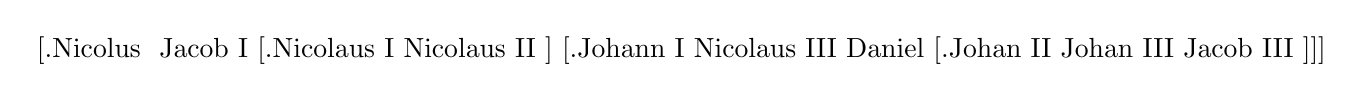
\begin{tikzpicture}
\node{\Tree 
 [.{Nicolus} { Jacob I}
    [.{Nicolaus I} {Nicolaus II}  ]
    [.{Johann I} {Nicolaus III} Daniel  [.{Johan II} {Johan III} {Jacob III} ]]]};%\\
\end{tikzpicture}
}


\begin{itemize}[label=\textbullet,noitemsep,nolistsep]
\item 8 mathematicians in the family. 120 disciples including Euler.
\item Jacob I solved problem of Isochrone curves. On this curve, ball from any height comes down in the same time. Cycloid takes min time than plane. Parabola takes most.
\item He also found ``Separation of Variables'' in Integration, Curve of a Sagging chain (Catenary), ``Logarithmic Spiral'' ($r=e^{a\theta}$),
\item Johann I was paid for a rule known as L'Hospital's rule.
\item Daniel was father of ``Mathematical Physics'' and worked on Hydraulics (Conversation of Energy), Theory of Vibrating Strings, Kinetic Theory of Gases etc.
\end{itemize}
\end{frame}

\begin{frame}[fragile]
\frametitle{Euler and Graph Theory}
\begin{itemize}[label=\textbullet,noitemsep,nolistsep]
\item Breathed Mathematics. Wrote beautifully and poetically. 
\item Number Theory, Mathematical Analysis, Astronomy, Light-Sound, Cartography, Graph Theory, Topology $\ldots$
\item Disciple of Johann I Bernoulli. Later overtook him. 
\item Proved that: In a network, with $ \geq 2$ odd vertices, its impossible to return to the original point without crossing any edge twice. Possible for $< 2$. K\"onigsberg bridges have 4 odd vertices, so cant come back.
\item Euler Path: Can trace edge only ones but need not come back. Possible for $\leq 2$ odd points, but not for $> 2$.
\item Graph Theory:`` Network formula'' Invariant $v + f = e + 1$
\item For Polyhedrons: $v -e + f = 2$. Birth of Topology.
\end{itemize}
\end{frame}

\begin{frame}[fragile]
\frametitle{Euler: an Architect of Mathematics}
\begin{itemize}[label=\textbullet,noitemsep,nolistsep]
\item Wrote ``The Elements of Algebra'', had Number theory.
\item Euler's constant $e$. Depicts Exponential Growth $y=e^x$. $e= \lim \limits_{n \to \infty} (1+\frac{1}{n})^n =2.71\ldots$
\item Discovered $e^{i \pi}+1=0$ and $e^{ix}=\cos{x} + i\sin{x}$
\item Literally lived mathematics. Won Paris Academy price 12 times. But in turn lost eyesight of one eye.
\item Wrote textbooks, on tides, chemistry, geography and also Mathematics in Music. About 75 volumes of 300-600 pages each. Plus 3000+ pages notes. $\frac{1}{3}$ of all the Mathematics, Mechanics in last 75 years of 18th century.
\end{itemize}
\end{frame}


\begin{frame}[fragile]
\frametitle{Lagrange: a Humble, Savant Mathematician}
\begin{itemize}[label=\textbullet,noitemsep,nolistsep]
\item ``Calculus of Variations'' (Geodesic: distance on a surface, Min-Max of functions etc), Number Theory, Differential Equations, Numerical Analysis (Bisection method).
\item Found definitive solution to $x^2-ny^2=1$ by method of ``Continued Fraction''. One equation with two variables - not possible. For certain $n$ you can get pairs of $x$ and $y$.
\end{itemize}
\end{frame}

\begin{frame}[fragile]
\frametitle{Lagrange and Laplace}
\begin{itemize}[label=\textbullet,noitemsep,nolistsep]
\item Stepping ahead of Newton and Leibniz (who used calculus to find rate of change), Laplace found ``Differential Equations'' (rate of change depends on variables e.g. $\frac{dy}{dx}=x$). $\frac{\partial x}{\partial y}$ for Partial Differential.
\item ``Treaties on Celestial Mechanics'' is considered next part of the ``Principia Mathematica''. Motion of planets.
\item Laplace wrote ``Meccanica Analitica'' (Analytical Mechanics). $E_{total} = E_{potetnial} + E_{kinetic}$. Had 4th dimension as `time'. Hated geometry so mostly equations.
\item Lagrange started decimal (Metric) system for measures.
\end{itemize}
\end{frame}

\begin{frame}[fragile]
\frametitle{Monge: New Pathways in Mathematics}
\begin{itemize}[label=\textbullet,noitemsep,nolistsep]
\item Started ``Projective Geometry''. For everyday use.
\item Founded ``Engineering Drawing'', ``Differential Geometry''.  Building machines, structures made possible.
\item ``Descriptive Geometry'': 2D projections/views of 3D.
\item Wrote ``Application de l'analyse \'a la g\'eom\'etrie''. Line on Curved Surface. Was later called as ``Non-Euclidean Geometry'' or "Riemann Geometry''.
\item Worked on Matrices, which are used in ``Finite Element Analysis''.
\item Wrote ``Art of Manufacturing Canon''!! 
\end{itemize}
\end{frame}

\begin{frame}[fragile]
\frametitle{Monge-Fourier: Victims of King-friendship}
\begin{itemize}[label=\textbullet,noitemsep,nolistsep]
\item By 14, consumed all 6 volumes by B\'ezu. Won prizes.
\item Changed Education system which was based on cramming, reciting notes. Started Q\&A dialogs in class.
\item Wrote first paper ``On Propagation of Heat in Solid Bodies'', reviewed by Monge, Laplace, Lagrange.
\item In the book ``The Analytical Theory of Heat'' he mentioned that ``any periodic function can be presented by sum of sines and cosines'', called ``Fourier Series''. $ f(x) = \frac{a_0}{2} + \sum \limits^{\infty}_{n=1} a_n cos(nx) + b_n sin(nx)$. Used in Signal Processing, or any phenomenon showing periodicity.
\item Representation of Discontinuous Curves by equations.
\end{itemize}
\end{frame}

\begin{frame}[fragile]
\frametitle{Carl Gauss: The Emperor of Mathematics}
\begin{itemize}[label=\textbullet,noitemsep,nolistsep]
\item Considered equivalent to Archimedes and Newton.
\item Toppled 2000 years old Euclidean Geometry.
\item Major mistake was that he kept his work a secret.
\item Laid foundation of ``Modular Mathematics'' (Clock Mathematics, as, e.g. 16 hrs, is actually 4pm, with periodicity of 12 hours. $ 16 = 4 \mod 12$). Security apps.
\item ``Method of Least Squares'' to fit a curve between points.
\item Instead of predicting Primes, tried their occurrences in given ranges. From $1 \rightarrow n = \frac{n}{\log_e{n}}$
\end{itemize}
\end{frame}

\begin{frame}[fragile]
\frametitle{Carl Gauss: A Scientist}
\begin{itemize}[label=\textbullet,noitemsep,nolistsep]
\item Predicted position of planet ``Ceres Ferdinandea'' using Newton's ``Inverse Square Law''.  Became a star at 24.
\item Napoleon spared G\"ottingen as Gauss was director there.
\item Strong memory, had Logarithm Tables by heart.
\item 4 Phases: Arithmetic till 1800, Astronomy up-to 1820, Geodesic and imaginary numbers till 1830 and Electromagnetism and light up-to 1840.
\end{itemize}
\end{frame}

\begin{frame}[fragile]
\frametitle{Abel and Quintic Equations}
\begin{itemize}[label=\textbullet,noitemsep,nolistsep]
\item Died at tender age of just 26. Fall of a glorious star.
\item Rewrote proofs by Newton, Euler, Gauss, Lagrange.
\item Proved which Quintic will have ``radical'' solution (factorization possible). Galois group over rationals.
\item Published 22 papers in first 3 editions of ``Crelle'' journal.
\item Found integrations for Transcendental functions.
\item Fourier opposed Able and Jacobi as their mathematics was not applied. But their Quintic is now used in Bose-Einstein Condensed state, Cosmology etc.
\end{itemize}
\end{frame}

\begin{frame}[fragile]
\frametitle{Rebellious Galois and Group Theory}
\begin{itemize}[label=\textbullet,noitemsep,nolistsep]
\item Died at 21. ``Remember my name!! My fate did not give me long enough life to do something extra-ordinary''
\item At 15, mastered Calculus, Analytical functions like a pro
\item Sensing his death he wrote all his invaluable mathematics. About 60 pages. Still not deciphered fully.
\item A ``Group'' (denoted by set $S$ and Operation $\oplus$) follows:
	\begin{itemize}[label=\textbullet,noitemsep,nolistsep]
	\item If $x,y \subset S$ then $ x \oplus y \subset S$. E.g $S$ has integers. $x=2,y=3$ and $\oplus$ is Addition, then $2+3=5 \subset S$
	\item If $x,y,z \subset S$ then $( x \oplus y) \oplus z = x \oplus (y \oplus z)$
	\item $S$ needs to have some Identity element $e$, so that $ x \oplus e = x$. $0$ for Addition, $1$ for Multiplication $\oplus$.
	\item for each $x$ there exists an inverse element $x'$ so that $x \oplus x' = e$. $-x$ for Addition, $\frac{1}{x}$ for Multiplication.
	\end{itemize}
\item ``All integers with Addition'' is a group but ``Integers from 1 to 10 and Multiplication' is not (Rule 1).
\end{itemize}
\end{frame}


\begin{frame}[fragile]
\frametitle{Foundations of Non-Euclidean Geometry}
\begin{itemize}[label=\textbullet,noitemsep,nolistsep,leftmargin=*]
\item Ancient geometry by Babylonians, Egyptians, Indians was 2D-Planar. Measuring land, building pyramids etc.
\item 13 volumes of ``The Elements'' by Euclid in 300 BC laid the foundation. Based 465 theorems on 5 postulates and 5 common notions. %Things which are self-evident, and independent, are called ``axioms'' (or postulates). 
	\begin{itemize}
	\item[1.] A straight line segment can be drawn between two points.
	\item[2.] Any straight line segment can be extended indefinitely.
	\item[3.] A circle can be drawn having the segment as radius and one endpoint as center.
	\item [4.] All right angles are congruent.
	\item [5.] If two lines with the sum of the inner angles less than 180, then they intersect if extended far enough.
	\end{itemize}
\item 
Euclid's fifth postulate cannot be proven as a theorem, although this was attempted by many people
\item On Curved surface, parallel lines meet. Sum of internal angles is more than 180, as each of base angle was 90.
\end{itemize}
\end{frame}

\begin{frame}[fragile]
\frametitle{Lobachevsky and Bolyai: Pioneers of the new-age Geometry}
\begin{itemize}[label=\textbullet,noitemsep,nolistsep]
\item Lobachevsky changed Euclid's 5th postulate to create self-consistent Non-Euclidean geometry
\item Became director of Kazan Univ at a young age. Toiled to make it prosperous. Good administrator. Hard working.
\item  Bolyai wrote 26 page paper ``Science of Absolute Space''
\item According to Euclid, one line can be drawn parallel to a given line at a point outside. According to Lobachevsky and Bolyai, mutiple and according to Rheimann, none.
\item Hermann Grassmann developed n-dimensional geometry.
\end{itemize}
\end{frame}



\begin{frame}[fragile]
\frametitle{Riemann: Mathematical wealth of an impoverished}
\begin{itemize}[label=\textbullet,noitemsep,nolistsep]
\item Finished Legendre's 859 pages book on numbers and logarithms in just 6 days. Could recollect after 2 years.
\item Like Euclid, own definitions of point, line and plane.
\item On Curved surface, line between two points, not unique.
\item Distances between points depend on curvature of surface
\item Metric Tensor for distances . Differential Geometry. 
\end{itemize}
\end{frame}


\begin{frame}[fragile]
\frametitle{Riemann, Hilbert and Hardy: Zeta functions}
\begin{itemize}[label=\textbullet,noitemsep,nolistsep]
\item Hilbert's 23 ``Unsolved Problems in Mathematics'' had ``Fermat's Last Theorem'' and Zeta functions were 8th
\item $\zeta(x) = \sum \limits_{n = 1}^{\infty} \frac{1}{n^x}$, with $x=1$ is a divergent series. Riemann found $\zeta (2) = \frac{\pi^2}{6}$. For $x=4,6$, in terms of $\pi^4, \pi^6$. But could not still find $\zeta (3),\zeta (5),\zeta (7)$. Not for negative $x$.
\item Hilbert's doctoral thesis on ``Theory of Invariants''. Redeveloped Euclid's geometry to propose 21 hypothesis. 
\item Einstein got help from Hilbert in the ``General Theory of Relativity'' and never denied it also.
\item At Trinity, Hardy and Littlewood wrote 100 papers.
\end{itemize}
\end{frame}


\begin{frame}[fragile]
\frametitle{Poincar\'e and Topology}
\begin{itemize}[label=\textbullet,noitemsep,nolistsep]
\item Algebra, Analysis, Geometry, Astronomy, Mathematical Physics etc. 100s of volumes. Brought diagrams back.
\item Doctorate under Hermite on Differential Equations.
\item Descartes saw Geometry as Algebra, Poincar\'e, opposite.
\item Topological equivalence is not on exact shape but connectivity, holes etc. Homeomorphism. Sphere-Cube, Cup-Donut are equivalent. Deformable. Rubber Sheet.
\item ``Ancient Utility Problem'': Connect 3 houses and 3 utilities without crossing. Not possible in 2D (provable by Jordan Curve theorem) but easier in 3D. Just lift.
\item ``Theory of Knots'': Started by Vandermonde as part of ``Geometry of Positions''. Shapes, weights irrelevant.
\item Tait's Conjectures: Alternating knots with 7 crossings.
\end{itemize}
\end{frame}


\begin{frame}[fragile]
\frametitle{Cantor: Set Theory and Infinity}
\begin{itemize}[label=\textbullet,noitemsep,nolistsep]
\item Infinity is an old concept. In ``Yajurveda'': infinity remains infinity even after taking something out of it.
\item Galileo's Paradox: Whole numbers are infinite and seemingly higher Natural numbers are also infinite. ``More'' infinite? Bolzano's ``Paradoxes of Infinity''.
\item Solved Trigonometry problem, left by Dirichlet, Riemann.
\item Six papers on Set Theory in ``Mathematische  Annalen''.
\item Equivalence of Sets: Cardinality, 1-to-1 Correspondence.
\item Uncountable Infinite sets contain irrationals like $\sqrt 2$
\end{itemize}
\end{frame}

\begin{frame}[fragile]
\frametitle{Ramanujan: Cursed Angle}
\begin{itemize}[label=\textbullet,noitemsep,nolistsep]
\item Brought to light by Hardy, comparable to Newton, Euler.
\item Got solutions in dreams. wrote them after getting up.
\item Failed in College 4 times. Lost Scholarship. Ran away.
\item Value of $\pi$ upto 6 decimal places with $k=0$ in $\frac{1}{\pi} = \frac{2\sqrt 2}{9801} \sum \limits_{k=0}^{\infty} \frac{(4k)!(1103+26390k)}{(k!)^4396^{4k}}$. 14 places with $k=1$.
\item ``Highly Composite'': more factors than any previous. 24. Found 102 till 6746328388800 with 269 equations.
\item Youngest (age 31) to get fellowship of Royal Academy.
\item ``Congruence in the number of partitions'' with Hardy.
\item Taxi number 1729 is $12^3+1^3$ and  $10^3+9^3$. Lowest such.
\end{itemize}
\end{frame}


\begin{frame}[fragile]
\frametitle{Neumann, Nash and Game Theory}
\begin{itemize}[label=\textbullet,noitemsep,nolistsep]
\item  Game Theory started by \`Emile Borel. Later developed by Neumann for gambling. Made famous by Nash (movie ``Beautiful Mind''). Nobel for ``Nash Equilibrium''.
\item Contributed to Eniac computer. ``Standard Programs''.
\item Nash's doctorate ``Non-Cooperative Games''. 27 pages.
\item Game theory applicable in interaction games like Poker, Bridge but not in independent games like Gambling.
\item ``Prisoner's Dilemma'': Cooperation than selfishness.
\item ``Nash Equilibrium'': Strategies benefiting all, work.
\end{itemize}
\end{frame}

\begin{frame}[fragile]
\frametitle{Women Mathematicians}
\begin{itemize}[label=\textbullet,noitemsep,nolistsep]
\item Theona: 6th century BC. Disciple and wife of Pythagoras. 
\item Hypatia: 4th century AD. Apollonius's conics. Astronomical charts.  Unmarried. Was killed brutally.
\item Agnesi: Studied curve ``versiera'' aka ``Witch of Agnesi''.
\item Sophie Germain: Studied under male name ``Antoine-August Le Blanc''. Lagrange become her mentor-philosopher. Vibration of Elastic Plates.
\item Sonya Kovalevskaya: Doctorate in-absentia. Differential Equations. Saturn rings. Rigid body ``Kovalvesky Top''.
\item Emmi Noethor: Applications of ``Theory of Relativity''
\end{itemize}
\end{frame}

\begin{frame}[fragile]
\frametitle{Statistics}
\begin{itemize}[label=\textbullet,noitemsep,nolistsep]
\item ``There are lies, damn lies and Statistics''- Mark Twain
\item First scientific study was by John Graunt, for epidemics. Study showed patterns, convincing of reason, not luck.
\item Halley (Comet fame) synthesized data as Life Tables and found interesting inferences like 346 survived till 50 out of 710 alive at 6. Out of 242 alive at 60, 41 reached 80.
\item Measurements like heights, weights, behavioral traits follow ``Normal Distribution'' (Bell or Gaussian Curve)
\item Data characterized (summary) by Mean, Mode, Median
\item Standard Deviation shows how data is away from Mean
\item Correlation of two variables is none if 0, strong if 1 or -1
\end{itemize}
\end{frame}

\begin{frame}[fragile]
\frametitle{Probability}
\begin{itemize}[label=\textbullet,noitemsep,nolistsep]
\item Chance-Likelihood of an event happening is Probability.
\item Cardano wroe wrote ``On Casting the Die'' on gambling
\item ``Problem of Points'': Pascal and Fermat found probability of a player winning at an intermediate stage.
\item Kolmogorov formalized it by postulates and theorems
\item Independent-Separable events like tossing a coin. Dependant are like blue-red ball example. Multiplying individual probabilities at each stage gives final value.
\item Used in Insurance, Genetics, Mechanics,Physics etc.
\end{itemize}
\end{frame}

\begin{frame}[fragile]
\frametitle{Logic}
\begin{itemize}[label=\textbullet,noitemsep,nolistsep]
\item Syllogism by Aristotle: Deduction by two propositions.
\item Augustus De Morgan, George Boole, Gottlob Frege used operator notation in logic. Boolean Algebra - equations.
\item AND (Intersection), OR (Union), NOT (Complement)
\item Frege: ``Axiomatic Predicate Logic''. Predicate are properties of subject. ``is green'' of a ball. Russel collapsed Frege's 10 year work, by his paradox (Barber).
\end{itemize}
\end{frame}

\begin{frame}[fragile]
\frametitle{Epilogue}

\begin{itemize}[label=\textbullet,noitemsep,nolistsep]
\item Ancient Mathematics: Arithmetic, Algebra, Geometry
\item 15-17th century: Conics, Calculus, Logarithms
\item 18th century: Graph Theory, Differential Geometry
\item 19th century: Non-Euclidean Geometry, N-Dimensional
\item 20th century: Topology, Chaos, Fractals, Probability
\item Indians: Ashutosh Mukherjee (Algebraic Curves), Vishnu Naralikar (Riemann Geometry), Pralhad Vaidya (Matrix - Astronomy), D D Kosambi (Tensor Analysis), Harish Chandra (Lie Groups), Shriram Abhyankar (Singularities), Mahalanobis  (Statistics-Distance), Ravindra Kulkarni (Differential Geometry).
\end{itemize}
\end{frame}



